\section{Introduction}\label{sec-intro}
Software bugs play a major role in the history of spacecraft
accidents~\cite{Leveson2004}. Some mission-ending bugs, e.g. those due to
software updates, would have been difficult to prevent, but plain integer
overflows~\cite{bug-rocket} and incorrect unit
conversion~\cite{NASA:1999:Mars} should have been eradicated long ago.
This paper
combines known formal verification and programming languages techniques and presents
a formal verification approach for simple control tasks, such as satellite power
management, which are executed on a real processing core used in space missions.

% Alas, there is no silver bullet. Testing is supported by mature methodologies
% and frameworks, but does not provide the full correctness guarantee. General-purpose
% strongly-typed languages can be used to eliminate important classes of bugs, but
% are less familiar to software engineers and are often not suitable for highly
% resource-constrained microarchitectures used in space electronics. Formal modelling
% methods provide a systematic approach for developing complex systems in a
% correct-by-construction manner, but they are still at the bleeding-edge of
% computing science and can be difficult to apply to real-life systems.

% We believe the presented ideas are transferable to other domains with similar
% safety and resource requirements, e.g. biomedical applications.

\begin{figure}
\centerline{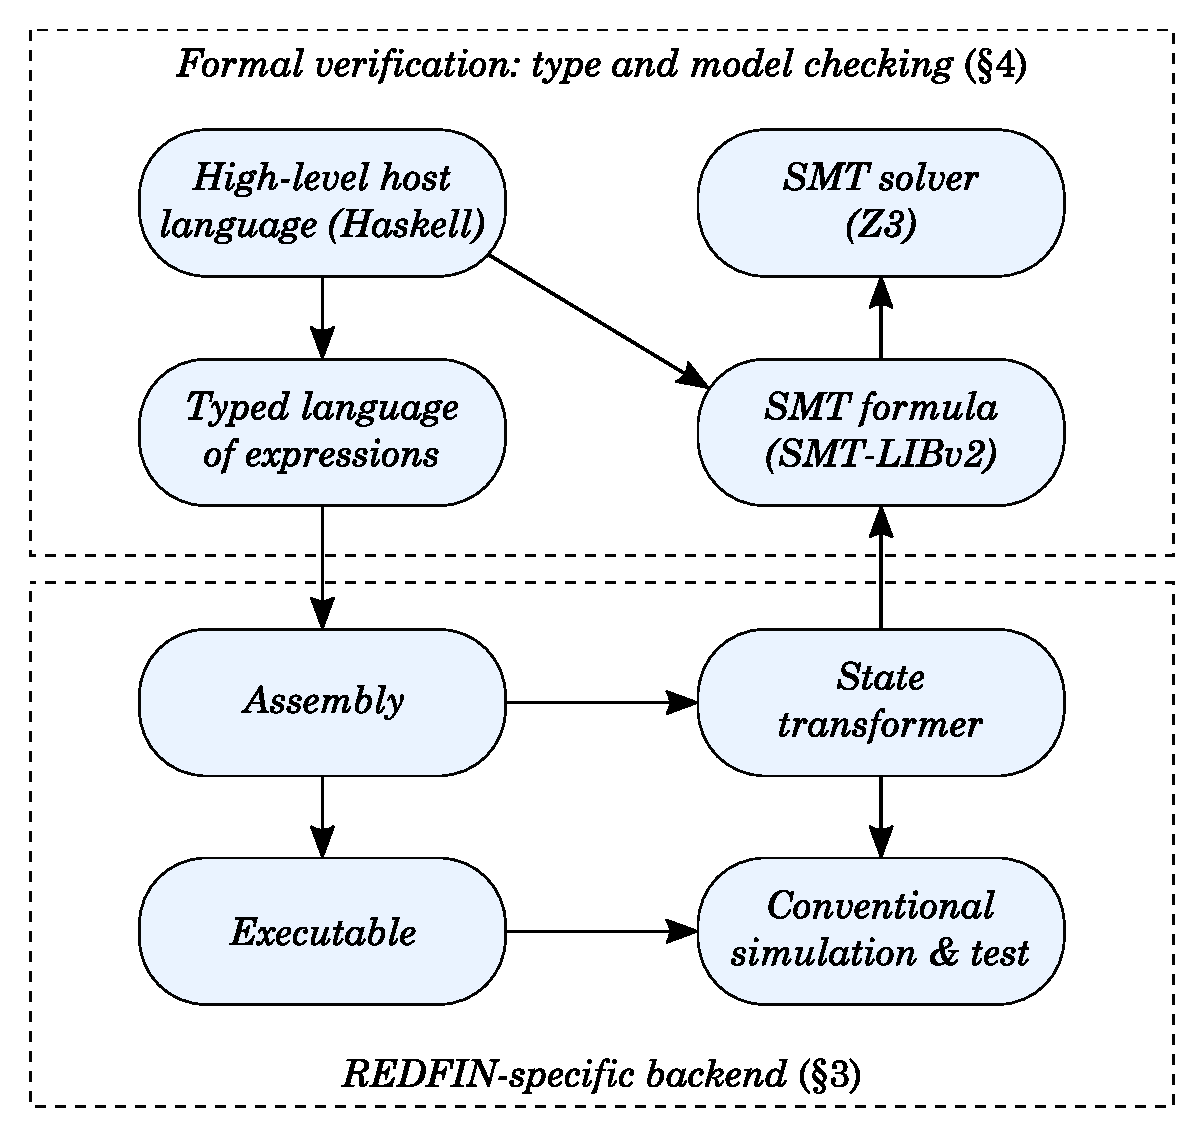
\includegraphics[scale=0.42]{fig/overview.pdf}}
\caption{Overview of the presented verification approach.\label{fig-overview}}
\Description[Please consult the text of this section for the description]{}
\end{figure}

Fig.~\ref{fig-overview} shows an overview of our approach. The bottom part
corresponds to conventional code generation and simulation, where
REDFIN\footnote{REDFIN stands for `REDuced instruction set for Fixed-point \&
INteger arithmetic'. This instruction set and the corresponding processing core
were developed by (Company Name) for space missions.
% RUAG Space Austria GmbH
See~\S\ref{sec-redfin} for more details.} assembly language is executed by
simulating the effect of each instruction on the state of the processor and memory.
The corresponding \emph{state transformer} is typically implicit and intertwined
with the rest of the simulation infrastructure. The main idea of our approach is
to represent the state transformer explicitly so that it can be symbolically
manipulated and used not only for simulation but also for formal verification.
The latter is achieved by compiling state transformers to SMT formulas and using
an SMT solver, e.g. Z3~\cite{de2008z3}, to verify that certain correctness
properties hold, for example, that integer overflow cannot occur regardless of
input parameters and that the program always terminates within stated time.

By using Haskell as the host language we can readily implement compilers from
higher-level \emph{typed} languages to untyped assembly, eradicating incorrect
number and unit conversion bugs. As shown at the top of Fig.~\ref{fig-overview},
engineers can write high-level control programs for the REDFIN architecture
directly in a small subset of Haskell. These high-level programs can be used for
type-safe code generation and as executable specifications of intended
functionality for the purposes of program synthesis and equivalence checking.

% To facilitate whole-program verification, we use a specific flavour of
% symbolic execution known as \emph{symbolic execution with merging}. In this approach,
% whenever a branch in the program is encountered, the symbolic execution engine performs
% merging of the two resulting disjunctive states, thus producing linear traces which could
% be translated into singular SMT-formulas representing whole programs. We refrain from a
% wider discussion of symbolic execution techniques here and refer the interested reader to
% the following survey paper~\cite{SurveySymExec-CSUR18}.

We first introduce the REDFIN processing core (\S\ref{sec-redfin}), then
present our verification approach (\S\ref{sec-transformer}-\S\ref{sec-verification}),
and conclude by a discussion (\S\ref{sec-discussion}) and a review of related
work (\S\ref{sec-related}).
